\documentclass{beamer}
\usefonttheme[onlymath]{serif}
\usepackage[T1]{fontenc}
\usepackage[utf8]{inputenc}
\usepackage[english]{babel}
\usepackage{amsmath}
\usepackage{amssymb}
\usepackage{amsthm}
\usepackage{gensymb}
\usepackage{parskip}
\usepackage{mathtools}
\usepackage{listings}
\usepackage{hyperref}
\usepackage{graphicx}
\usepackage{color}
\usepackage{enumerate}
\usepackage{tikz}
\usetikzlibrary{calc}
\usetikzlibrary{positioning}
\usetikzlibrary{angles}
\usetikzlibrary{shapes}
\usetikzlibrary{arrows}
\usepackage{verbatim}
\usepackage{multicol}
\usepackage{array}
\usepackage{minted}
\parskip 0pt


\DeclareMathOperator{\lcm}{lcm}
\newcommand\floor[1]{\left\lfloor#1\right\rfloor}
\newcommand\ceil[1]{\left\lceil#1\right\rceil}
\newcommand\abs[1]{\left|#1\right|}
\newcommand\p[1]{\left(#1\right)}
\newcommand\sqp[1]{\left[#1\right]}
\newcommand\cp[1]{\left\{#1\right\}}
\newcommand\norm[1]{\left\lVert#1\right\rVert}
\renewcommand\Im{\operatorname{Im}}
\renewcommand\Re{\operatorname{Re}}

\usetheme{metropolis}
\definecolor{dark yellow}{rgb} {0.6,0.6,0.0}
\definecolor{dark green}{rgb} {0.0,0.6,0.0}

\graphicspath{{myndir/}}

\title{Divide and conquer, Dynamic programming}
\author{Atli FF}
\institute{\href{http://ru.is/td}{School of Computer Science} \\[2pt] \href{http://ru.is}{Reykjavík University}}
\titlegraphic{\hfill
\includegraphics[height=0.6cm]{kattis}}

\begin{document}
\maketitle

\section{Divide and conquer}
\begin{frame}[plain]{Divide and conquer}
    \begin{itemize}
        \item Given an instance of the problem, the basic idea is to
        \begin{enumerate}
            \item split the problem into one or more smaller subproblems
            \item solve each of these subproblems recursively
            \item combine the solutions to the subproblems into a solution of the given problem
        \end{enumerate}

        \vspace{5pt}

        \item Some standard divide and conquer algorithms:
        \begin{itemize}
            \item Quicksort / Mergesort
            \item Karatsuba algorithm
            \item Strassen algorithm
            \item Many algorithms from computational geometry
                \begin{itemize}
                    \item Convex hull
                    \item Closest pair of points
                \end{itemize}
        \end{itemize}
    \end{itemize}
\end{frame}

\begin{frame}[plain,fragile]{Divide and conquer: Time complexity}
    \begin{minted}[fontsize=\scriptsize]{cpp}
void solve(int n) {
    if (n == 0)
        return;

    solve(n/2);
    solve(n/2);

    for (int i = 0; i < n; i++) {
        // some constant time operations
    }
}
    \end{minted}

    \begin{itemize}
        \item What is the time complexity of this divide and conquer algorithm?
        \item Usually helps to model the time complexity as a recurrence relation:
            \begin{itemize}
                \item $T(n) = 2T(n/2) + n$
            \end{itemize}
    \end{itemize}
\end{frame}

\begin{frame}[plain,fragile]{Divide and conquer: Time complexity}
    \begin{itemize}
        \item But how do we solve such recurrences?
        \item Usually simplest to use the Master theorem when applicable
            \begin{itemize}
                \item It gives a solution to a recurrence of the form $T(n) = aT(n/b) + f(n)$ in asymptotic terms
                \item All of the divide and conquer algorithms mentioned so far have a recurrence of this form
            \end{itemize}
        \vspace{10pt}
        \item The Master theorem tells us that $T(n) = 2T(n/2) + n$ has asymptotic time complexity $O(n \log n)$
        \vspace{10pt}
        \item You don't need to know the Master theorem for this course, but still recommended as it's very useful
    \end{itemize}
\end{frame}

\begin{frame}[plain]{Decrease and conquer}
    \begin{itemize}
        \item Sometimes we're not actually dividing the problem into many subproblems, but only into one smaller subproblem
        \item Usually called decrease and conquer
        \item The most common example of this is binary search
    \end{itemize}
\end{frame}

\begin{frame}[plain]{Binary search}
    \begin{itemize}
        \item We have a \textbf{sorted} array of elements, and we want to check if it contains a particular element $x$
        \vspace{5pt}
        \item Algorithm:
        \begin{enumerate}
            \item Base case: the array is empty, return false
            \item Compare $x$ to the element in the middle of the array
            \item If it's equal, then we found $x$ and we return true
            \item If it's less, then $x$ must be in the left half of the array
            \begin{enumerate}
                \item Binary search the element (recursively) in the left half
            \end{enumerate}
            \item If it's greater, then $x$ must be in the right half of the array
            \begin{enumerate}
                \item Binary search the element (recursively) in the right half
            \end{enumerate}
        \end{enumerate}
    \end{itemize}
\end{frame}

\begin{frame}[plain,fragile]{Binary search}
    \begin{minted}[fontsize=\scriptsize]{cpp}
bool binary_search(const vector<int> &arr, int lo, int hi, int x) {
    if (lo > hi) {
        return false;
    }

    int m = (lo + hi) / 2;
    if (arr[m] == x) {
        return true;
    } else if (x < arr[m]) {
        return binary_search(arr, lo, m - 1, x);
    } else if (x > arr[m]) {
        return binary_search(arr, m + 1, hi, x);
    }
}

binary_search(arr, 0, arr.size() - 1, x);
    \end{minted}

    \begin{itemize}
        \item $T(n) = T(n/2) + 1$
        \item $O(\log n)$
    \end{itemize}
\end{frame}

\begin{frame}[plain,fragile]{Binary search - iterative}
    \begin{minted}[fontsize=\scriptsize]{cpp}
bool binary_search(const vector<int> &arr, int x) {
    int lo = 0,
        hi = arr.size() - 1;

    while (lo <= hi) {
        int m = (lo + hi) / 2;
        if (arr[m] == x) {
            return true;
        } else if (x < arr[m]) {
            hi = m - 1;
        } else if (x > arr[m]) {
            lo = m + 1;
        }
    }

    return false;
}
    \end{minted}
\end{frame}

\begin{frame}[plain]{Binary search over integers}
    \begin{itemize}
        \item This might be the most well known application of binary search, but it's far from being the only application
        \item More generally, we have a predicate $p : \{0,\ldots,n-1\} \rightarrow \{T, F\}$ which has the property that if $p(i) = T$, then $p(j) = T$ for all $j > i$
        \item Our goal is to find the smallest index $j$ such that $p(j) = T$ as quickly as possible
    \end{itemize}

    \begin{center}
        \begin{tabular}{ccccccccccccccccccc}
            $i$ & $0$ & $1$ & $\cdots$ & $j-1$ & \color{blue}{$j$} & $j+1$ & $\cdots$ & $n-2$ & $n-1$ \\
            \hline
            $p(i)$ & $F$ & $F$ & $\cdots$ & $F$ & \color{blue}{$T$} & $T$ & $\cdots$ & $T$ & $T$ \\
        \end{tabular}
    \end{center}

    \begin{itemize}
        \item We can do this in $O(\log(n) \times f)$ time, where $f$ is the cost of evaluating the predicate $p$, in the same way as when we were binary searching an array
    \end{itemize}
\end{frame}

\begin{frame}[plain,fragile]{Binary search over integers}
    \begin{minted}[fontsize=\footnotesize]{cpp}
int lo = 0,
    hi = n - 1;

while (lo < hi) {
    int m = (lo + hi) / 2;

    if (p(m)) {
        hi = m;
    } else {
        lo = m + 1;
    }
}

if (lo == hi && p(lo)) {
    printf("lowest index is %d\n", lo);
} else {
    printf("no such index\n");
}
    \end{minted}
\end{frame}

\begin{frame}[plain,fragile]{Binary search over reals}
    \begin{itemize}
        \item An even more general version of binary search is over the real numbers
        \item We have a predicate $p : [lo,hi] \rightarrow \{T, F\}$ which has the property that if $p(i) = T$, then $p(j) = T$ for all $j > i$
        \item Our goal is to find the smallest real number $j$ such that $p(j) = T$ as quickly as possible

        \vspace{5pt}
        \item Since we're working with real numbers (hypothetically), our $[lo,hi]$ can be halved infinitely many times without ever becoming a single real number
        \item Instead it will suffice to find a real number $j'$ that is very close to the correct answer $j$, say not further than $EPS = 2^{-30}$ away, we can do this in $O(\log(\frac{hi - lo}{EPS}))$ time in a similar way as when we were binary searching an array
    \end{itemize}
\end{frame}

\begin{frame}[plain]{Example}
	\begin{center}
		\begin{tikzpicture}
			[domain = -0.2:4.2]
			\draw[->] (-0.2,0) -- (4.2,0);
			\draw[->] (0,-0.2) -- (0,4.2);
			\draw[color=red] plot[id=c] function{2} node[right] {$y$};
			\draw[color=blue] plot[id=poly3] function{0.9 + 1.08333*x - 0.75*x**2 + 0.166667*x**3} node[right] {$f(x)$};



			\node<all:1-2>[below] at (0.7,-0.125) {$a$};
			\draw<all:1-2> (0.7,0.125) -- (0.7,-0.125);
			\draw<all:1-2>[dashed, gray] (0.7,0.125) -- (0.7, 4.2);
			\node<all:1-6>[below] at (3.7,-0.125) {$b$};
			\draw<all:1-6>(3.7,0.125) -- (3.7,-0.125);
			\draw<all:1-6>[dashed, gray] (3.7,0.125) -- (3.7,4.2);

			\node<all:2>[below] at (2.2,-0.125) {$m$};
			\draw<all:2-4> (2.2,0.125) -- (2.2,-0.125);
			\draw<all:2-4>[dashed, gray] (2.2,0.125) -- (2.2,4.2);

			\node<all:3-4>[below] at (2.2,-0.125) {$a$};

			\node<all:4>[below] at (2.95,-0.125) {$m$};
			\draw<all:4-> (2.95,0.125) -- (2.95,-0.125);
			\draw<all:4->[dashed, gray] (2.95,0.125) -- (2.95,4.2);

			\node<all:5->[below] at (2.95,-0.125) {$a$};

			\node<all:6>[below] at (3.325,-0.125) {$m$};
			\draw<all:6-> (3.325,0.125) -- (3.325,-0.125);
			\draw<all:6->[dashed, gray] (3.325,0.125) -- (3.325,4.2);

			\node<all:7->[below] at (3.325,-0.125) {$b$};
        \end{tikzpicture}
    \end{center}
\end{frame}

\begin{frame}[plain,fragile]{Binary search over reals}
    \begin{minted}{cpp}
double EPS = 1e-10,
       lo = -1000.0,
       hi = 1000.0;

while (hi - lo > EPS) {
    double mid = (lo + hi) / 2.0;

    if (p(mid)) {
        hi = mid;
    } else {
        lo = mid;
    }
}

printf("%0.10lf\n", lo);
    \end{minted}
\end{frame}

\begin{frame}[plain,fragile]{Binary search over reals}
    \begin{itemize}
        \item This has many cool numerical applications
        \vspace{5pt}
        \item Find the square root of $x$
    \end{itemize}
    \begin{minted}{cpp}
bool p(double j) {
    return j*j >= x;
}
    \end{minted}
    \begin{itemize}
        \item Find the root of an increasing function $f(x)$
    \end{itemize}
    \begin{minted}{cpp}
bool p(double x) {
    return f(x) >= 0.0;
}
    \end{minted}

    \begin{itemize}
        \item This is also referred to as the Bisection method
    \end{itemize}
\end{frame}

\begin{frame}[plain]{Binary search the answer}
    \begin{itemize}
        \item It may be hard to find the optimal solution directly, as we saw in the example problem
        \item On the other hand, it may be easy to check if some $x$ is a solution or not
        \vspace{5pt}
        \item A method of using binary search to find the minimum or maximum solution to a problem
        \item Only applicable when the problem has the binary search property: if $i$ is a solution, then so are all $j > i$
        \vspace{5pt}
        \item $p(i)$ checks whether $i$ is a solution, then we simply apply binary search on $p$ to get the minimum or maximum solution
    \end{itemize}
\end{frame}

\begin{frame}[plain]{Ternary search}
    \begin{itemize}
        \item Another useful and similar algorithm is ternary search
        \item This time we have a convex function $f$ ($f'' \geq 0$), so it might decrease at first and then increase
        \item This function will have a unique minimum value that we might want to find, perhaps to minimize some cost function
        \item This can be done in a similar fashion to binary search
    \end{itemize}
\end{frame}

\begin{frame}[plain]{Ternary search}
	\begin{itemize}
        \item We choose points $m_1, m_2$ in our interval $[a, b]$ so $[a, m_1]$, $[m_1, m_2]$ and $[m_2, b]$ are equally large.
        \item We then consider $f(m_1), f(m_2)$.
        \item If $f(m_1) < f(m_2)$ the minimum can not be in $[m_2, b]$ so we can discard it.
        \item If $f(m_2) < f(m_1)$ the minimum can not be in $[a, m_1]$ so we can discard it.
        \item If $f(m_1) = f(m_2)$ the minimum must be in $[m_1, m_2]$.
        \item This can be shown to be true using analysis, since convex functions take their maxima on the endpoints of intervals.
    \end{itemize}
\end{frame}

\begin{frame}{Example}
	\begin{center}
		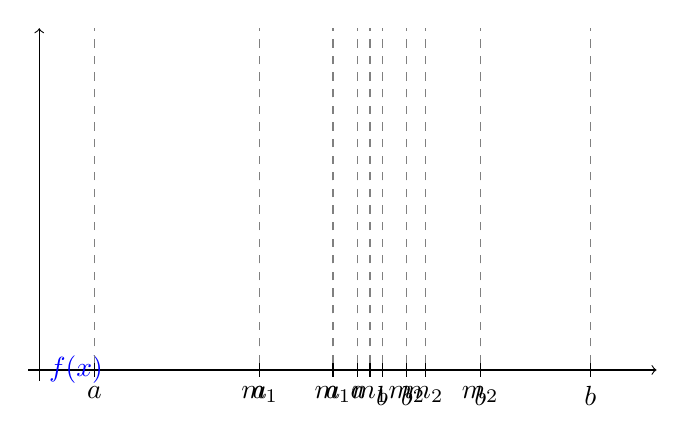
\begin{tikzpicture}[scale = 0.7, domain=-0.2:11.2]
			\draw[->] (-0.2,0) -- (11.2,0);
			\draw[->] (0,-0.2) -- (0,6.2);
			\draw[color = blue] plot[id=poly2] function{5 - 1.2*x + 0.1*x**2} node[right] {$f(x)$};

			\node<all:1-2>[below] at (1,-0.125) {$a$};
			\draw<all:1-2> (1,0.125) -- (1,-0.125);
			\draw<all:1-2>[dashed, gray] (1,0.125) -- (1, 6.2);

			\node<all:1-4>[below] at (10,-0.125) {$b$};
			\draw<all:1-4>(10,0.125) -- (10,-0.125);
			\draw<all:1-4>[dashed, gray] (10,0.125) -- (10,6.2);

			\node<all:2>[below] at (4,-0.125) {$m_1$};
			\draw<all:2>(4,0.125) -- (4,-0.125);
			\draw<all:2>[dashed, gray] (4,0.125) -- (4,6.2);

			\node<all:2>[below] at (7,-0.125) {$m_2$};
			\draw<all:2>(7,0.125) -- (7,-0.125);
			\draw<all:2>[dashed, gray] (7,0.125) -- (7,6.2);

			\node<all:3-6>[below] at (4,-0.125) {$a$};
			\draw<all:3-6> (4,0.125) -- (4,-0.125);
			\draw<all:3-6>[dashed, gray] (4,0.125) -- (4, 6.2);

			\node<all:4>[below] at (6,-0.125) {$m_1$};
			\draw<all:4>(6,0.125) -- (6,-0.125);
			\draw<all:4>[dashed, gray] (6,0.125) -- (6,6.2);

			\node<all:4>[below] at (8,-0.125) {$m_2$};
			\draw<all:4>(8,0.125) -- (8,-0.125);
			\draw<all:4>[dashed, gray] (8,0.125) -- (8,6.2);

			\node<all:5-6>[below] at (8,-0.125) {$b$};
			\draw<all:5-6>(8,0.125) -- (8,-0.125);
			\draw<all:5-6>[dashed, gray] (8,0.125) -- (8,6.2);

			\node<all:6>[below] at (5.33,-0.125) {$m_1$};
			\draw<all:6>(5.33,0.125) -- (5.33,-0.125);
			\draw<all:6>[dashed, gray] (5.33,0.125) -- (5.33,6.2);

			\node<all:6>[below] at (6.67,-0.125) {$m_2$};
			\draw<all:6>(6.67,0.125) -- (6.67,-0.125);
			\draw<all:6>[dashed, gray] (6.67,0.125) -- (6.67,6.2);

			\node<all:7-8>[below] at (5.33,-0.125) {$a$};
			\draw<all:7-8>(5.33,0.125) -- (5.33,-0.125);
			\draw<all:7-8>[dashed, gray] (5.33,0.125) -- (5.33,6.2);

			\node<all:7-8>[below] at (6.67,-0.125) {$b$};
			\draw<all:7-8>(6.67,0.125) -- (6.67,-0.125);
			\draw<all:7-8>[dashed, gray] (6.67,0.125) -- (6.67,6.2);

			\draw<all:8>(5.78,0.125) -- (5.78,-0.125);
			\draw<all:8>[dashed, gray] (5.78,0.125) -- (5.78,6.2);

			\draw<all:8>(6.22,0.125) -- (6.22,-0.125);
			\draw<all:8>[dashed, gray] (6.22,0.125) -- (6.22,6.2);

			\node<all:9>[below] at (5.78,-0.125) {$a$};
			\draw<all:9>(5.78,0.125) -- (5.78,-0.125);
			\draw<all:9>[dashed, gray] (5.78,0.125) -- (5.78,6.2);

			\node<all:9>[below] at (6.22,-0.125) {$b$};
			\draw<all:9>(6.22,0.125) -- (6.22,-0.125);
			\draw<all:9>[dashed, gray] (6.22,0.125) -- (6.22,6.2);
		\end{tikzpicture}
    \end{center}
\end{frame}

\begin{frame}[plain,fragile]{Binary exponentiation}
    \begin{itemize}
        \item We want to calculate $x^n$, where $x,n$ are integers
        \item Assume we don't have the built-in \texttt{pow} method
        \item Naive method:
    \end{itemize}

    \begin{minted}{cpp}
int pow(int x, int n) {
    int res = 1;
    for (int i = 0; i < n; i++) {
        res = res * x;
    }

    return res;
}
    \end{minted}

    \begin{itemize}
        \item This is $O(n)$, but what if we want to support large $n$ efficiently?
    \end{itemize}
\end{frame}

\begin{frame}[plain]{Binary exponentiation}
    \begin{itemize}
        \item Let's use divide and conquer
        \vspace{10pt}
        \item Notice the three identities:

            \begin{itemize}
                \item $x^0 = 1$
                \item $x^n = x \times x^{n-1}$
                \item $x^n = x^{n/2} \times x^{n/2}$
            \end{itemize}

        \item Or in terms of our function:

            \begin{itemize}
                \item $pow(x,0) = 1$
                \item $pow(x,n) = x \times pow(x, n-1)$
                \item $pow(x,n) = pow(x, n/2) \times pow(x, n/2)$
            \end{itemize}

        \item $pow(x,n/2)$ is used twice, but we only need to compute it once:

            \begin{itemize}
                \item $pow(x,n) = pow(x, n/2)^2$
            \end{itemize}
    \end{itemize}
\end{frame}

\begin{frame}[plain,fragile]{Binary exponentiation}
    \begin{itemize}
        \item Let's try using these identities to compute the answer recursively
    \end{itemize}

    \vspace{10pt}

    \begin{minted}{cpp}
int pow(int x, int n) {
    if (n == 0) return 1;
    return x * pow(x, n - 1);
}
    \end{minted}

    \vspace{10pt}

    \begin{itemize}
        \item<2-> How efficient is this?
            \begin{itemize}
                \item $T(n) = 1 + T(n-1)$
                \item<3-> $O(n)$
                \item<4-> Still just as slow...
            \end{itemize}
    \end{itemize}

\end{frame}

\begin{frame}[plain,fragile]{Binary exponentiation}
    \begin{itemize}
        \item What about the third identity?
            \begin{itemize}
                \item $n/2$ is not an integer when $n$ is odd, so let's only use it when $n$ is even
            \end{itemize}
    \end{itemize}

    \begin{minted}{cpp}
int pow(int x, int n) {
    if (n == 0) return 1;
    if (n % 2 != 0) return x * pow(x, n - 1);
    int st = pow(x, n/2);
    return st * st;
}
    \end{minted}

    \begin{itemize}
        \item How efficient is this?
            \begin{itemize}
                \item<2-> $T(n) = 1 + T(n-1)$ if $n$ is odd
                \item<2-> $T(n) = 1 + T(n/2)$ if $n$ is even
                \item<3-> $T(n) = 1 + 1 + T((n-1)/2)$ if $n$ is odd
                \item<4-> $O(\log n)$
            \end{itemize}
    \end{itemize}
\end{frame}

\begin{frame}[plain]{Binary exponentiation}
    \begin{itemize}
        \item Notice that $x$ doesn't have to be an integer, and $\star$ doesn't have to be integer multiplication...
        \item It also works for:
            \begin{itemize}
                \item Computing $x^n$, where $x$ is a floating point number and $\star$ is floating point number multiplication
                \item Computing $A^n$, where $A$ is a matrix and $\star$ is matrix multiplication
                \item Computing $x^n \pmod{m}$, where $x$ is an integer and $\star$ is integer multiplication modulo $m$
                \item Computing $x\star x\star \cdots \star x$, where $x$ is any element and $\star$ is any associative operator
            \end{itemize}

        \item All of these can be done in $O(\log(n) \times f)$, where $f$ is the cost of doing one application of the $\star$ operator
    \end{itemize}
\end{frame}

\begin{frame}[plain]{Fibonacci words}
    \begin{itemize}
        \item Recall that the Fibonacci sequence can be defined as follows:
            \begin{itemize}
        \item $\mathrm{fib}_1 = 1$
        \item $\mathrm{fib}_2 = 1$
        \item $\mathrm{fib}_n = \mathrm{fib}_{n-2} + \mathrm{fib}_{n-1}$
            \end{itemize}
        \item We get the sequence $1, 1, 2, 3, 5, 8, 13, 21, \ldots$
        \item There are many generalizations of the Fibonacci sequence
        \item One of them is to start with other numbers, like:
            \begin{itemize}
                \item $f_1 = 5$
                \item $f_2 = 4$
                \item $f_n = f_{n-2} + f_{n-1}$
            \end{itemize}
        \item We get the sequence $5, 4, 9, 13, 22, 35, 57, \ldots$
        \item What if we start with something other than numbers?
    \end{itemize}
\end{frame}

\begin{frame}[plain]{Fibonacci words}
    \begin{itemize}
        \item Let's try starting with a pair of strings, and let $+$ denote string concatenation:
            \begin{itemize}
                \item $g_1 = A$
                \item $g_2 = B$
                \item $g_n = g_{n-2} + g_{n-1}$
            \end{itemize}
        \vspace{10pt}
        \item Now we get the sequence of strings:
        \begin{align*}
        &A, B, AB, BAB, ABBAB, BABABBAB, \\
        &ABBABBABABBAB, \\
        &BABABBABABBABBABABBAB, \ldots \\
        \end{align*}
    \end{itemize}
\end{frame}

\begin{frame}[plain]{Fibonacci words}
    \begin{itemize}
        \item How long is $g_n$?
        \begin{itemize}
            \item $\mathrm{len}(g_1) = 1$
            \item $\mathrm{len}(g_2) = 1$
            \item $\mathrm{len}(g_n) = \mathrm{len}(g_{n-2}) + \mathrm{len}(g_{n-1})$
        \end{itemize}
        \vspace{5pt}
        \item Looks familiar?
        \vspace{2pt}
        \item $\mathrm{len}(g_n) = \mathrm{fib}_{n}$
        \vspace{10pt}
        \item So the strings become very large very quickly
        \begin{itemize}
            \item $\mathrm{len}(g_{10}) = 55$
            \item $\mathrm{len}(g_{100}) = 354224848179261915075$
        \end{itemize}
    \end{itemize}
\end{frame}

\begin{frame}[plain]{Fibonacci words}
    \begin{itemize}
        \item Task: Compute the $i$th character in $g_{n}$
        \vspace{10pt}
        \item<2-> Simple to do in $O(\mathrm{len}(n))$, but that is extremely slow for large $n$
        \vspace{10pt}
        \item<3-> Can be done in $O(n)$ using divide and conquer
    \end{itemize}
\end{frame}

\section*{Dynamic Programming}

\begin{frame}[plain]{What is dynamic programming?}
    \begin{itemize}
        \item A problem solving paradigm
        \item Similar in some respects to both divide and conquer and backtracking
        \vspace{5pt}
        \item Divide and conquer recap:
        \begin{itemize}
            \item Split the problem into \textit{independent} subproblems
            \item Solve each subproblem recursively
            \item Combine the solutions to subproblems into a solution for the given problem
        \end{itemize}
        \vspace{5pt}
        \item Dynamic programming:
        \begin{itemize}
            \item Split the problem into \textit{overlapping} subproblems
            \item Solve each subproblem recursively
            \item Combine the solutions to subproblems into a solution for the given problem
            \item \textit{Don't compute the answer to the same subproblem more than once}
        \end{itemize}
    \end{itemize}
\end{frame}

\begin{frame}[plain,fragile]{Dynamic programming formulation}
    \vspace{30pt}
    \begin{itemize}
        \item Formulate the problem in terms of smaller versions of the problem (recursively)
        \item Turn this formulation into a recursive function
        \item Memoize the function (remember results that have been computed)
    \end{itemize}
\end{frame}

\begin{frame}[plain,fragile]{Dynamic programming formulation}
    \begin{minted}[fontsize=\footnotesize]{cpp}
map<problem, value> memory;

value dp(problem P) {
    if (is_base_case(P)) {
        return base_case_value(P);
    }

    if (memory.find(P) != memory.end()) {
        return memory[P];
    }

    value result = some value;
    for (problem Q in subproblems(P)) {
        result = combine(result, dp(Q));
    }

    memory[P] = result;
    return result;
}
    \end{minted}
\end{frame}

\begin{frame}[plain]{The Fibonacci sequence}
    \vspace{5pt}
    \textit{The first two numbers in the Fibonacci sequence are 1 and 1. All
            other numbers in the sequence are defined as the sum of the previous two
            numbers in the sequence.}

    \vspace{5pt}
    \begin{itemize}
        \item Task: Find the $n$th number in the Fibonacci sequence
        \item Let's solve this with dynamic programming
    \end{itemize}

    \vspace{5pt}
    \begin{itemize}
        \item Formulate the problem in terms of smaller versions of the problem (recursively)
    \end{itemize}

    \begin{align*}
        \mathrm{fibonacci}(1) &= 1\\
        \mathrm{fibonacci}(2) &= 1\\
        \mathrm{fibonacci}(n) &= \mathrm{fibonacci}(n - 2) + \mathrm{fibonacci}(n - 1)
    \end{align*}
\end{frame}

\begin{frame}[plain,fragile]{The Fibonacci sequence}
    \begin{itemize}
        \item[2.] Turn this formulation into a recursive function
    \end{itemize}

    \begin{minted}[fontsize=\footnotesize]{cpp}
int fibonacci(int n) {
    if (n < 2) {
        return n;
    }

    int res = fibonacci(n - 2) + fibonacci(n - 1);

    return res;
}
    \end{minted}
\end{frame}

\begin{frame}[plain,fragile]{The Fibonacci sequence}
    \begin{itemize}
        \item What is the time complexity of this? \onslide<2->{Exponential, almost $O(2^n)$}
    \end{itemize}

    \begin{figure}

        \begin{tikzpicture}

[-,thick,%
  every node/.style={shape=circle,draw,thick},%
  level distance=0.5cm,
  growth parent anchor={south}, nodes={anchor=north},
  scale=0.8,%
]
\scriptsize
\node {$fib(6)$}
  [sibling distance=5cm]
  child {node {$fib(4)$}
    [sibling distance=2cm]
    child {node {$fib(2)$}
    }
    child {node {$fib(3)$}
      [sibling distance=1cm]
      child {node {$fib(1)$}
        [sibling distance=0.5cm]
      }
      child {node {$fib(2)$}
      }
    }
  }
  child {node {$fib(5)$}
    [sibling distance=3cm]
    child {node {$fib(3)$}
      [sibling distance=1cm]
      child {node {$fib(1)$}
        [sibling distance=0.5cm]
      }
      child {node {$fib(2)$}
          }
    }
    child {node {$fib(4)$}
      [sibling distance=2cm]
      child {node {$fib(2)$}
      }
      child {node {$fib(3)$}
        [sibling distance=1cm]
        child {node {$fib(1)$}
          [sibling distance=0.5cm]
        }
        child {node {$fib(2)$}
        }
      }
    }
  };
        \end{tikzpicture}
    \end{figure}
\end{frame}

\begin{frame}[plain,fragile]{The Fibonacci sequence}
    \begin{itemize}
        \item[3.] Memoize the function (remember results that have been computed)
    \end{itemize}

    \vspace{5pt}

    \begin{minted}[fontsize=\footnotesize]{cpp}
map<int, int> mem;

int fibonacci(int n) {
    if (n <= 2) {
        return 1;
    }

    if (mem.find(n) != mem.end()) {
        return mem[n];
    }

    int res = fibonacci(n - 2) + fibonacci(n - 1);

    mem[n] = res;
    return res;
}
    \end{minted}

\end{frame}

\begin{frame}[plain,fragile]{The Fibonacci sequence}
    \vspace{5pt}

    \begin{minted}[fontsize=\footnotesize]{cpp}
int mem[1000];
for (int i = 0; i < 1000; i++)
    mem[i] = -1;

int fibonacci(int n) {
    if (n <= 2) {
        return 1;
    }

    if (mem[n] != -1) {
        return mem[n];
    }

    int res = fibonacci(n - 2) + fibonacci(n - 1);

    mem[n] = res;
    return res;
}
    \end{minted}

\end{frame}

\begin{frame}[plain]{The Fibonacci sequence}
    \begin{itemize}
        \item What is the time complexity now?
        \vspace{5pt}
        \item We have $n$ possible inputs to the function: $1$, $2$, \ldots, $n$.
        \item Each input will either:
            \begin{itemize}
                \item be computed, and the result saved
                \item be returned from memory
            \end{itemize}
        \item Each input will be computed at most once
        \item Time complexity is $O(n \times f)$, where $f$ is the time complexity of computing an input if we assume that the recursive calls are returned directly from memory ($O(1)$)
        \item Since we're only doing constant amount of work to compute the answer to an input, $f = O(1)$
        \item Total time complexity is $O(n)$
    \end{itemize}
\end{frame}

\begin{frame}[plain]{Maximum sum}

    \vspace{10pt}

    \begin{itemize}
\item Given an array $\mathrm{arr}[0]$, $\mathrm{arr}[1]$, \ldots, $\mathrm{arr}[n-1]$ of integers, find the interval with the highest sum
    \end{itemize}

    \begin{center}
        \begin{tabular}{|c|c|c|c|c|c|c|}
            \hline
            -15 & \color<2->{blue}{8} & \color<2->{blue}{-2} & \color<2->{blue}{1} & \color<2->{blue}{0} & \color<2->{blue}{6} & -3 \\
            \hline
        \end{tabular}
    \end{center}

    \begin{itemize}
        \item<2-> The maximum sum of an interval in this array is $13$

        \item<3-> But how do we solve this in general?
            \begin{itemize}
        \item Easy to loop through all $\approx n^2$ intervals, and calculate their sums, but that is $O(n^3)$
        \item We could use our static range sum trick to get this down to $O(n^2)$
        \item Can we do better with dynamic programming?
            \end{itemize}
    \end{itemize}

\end{frame}

\begin{frame}[plain]{Maximum sum}

    \vspace{20pt}

    \begin{itemize}
        \item First step is to formulate this recursively
        \vspace{5pt}
        \item Let $\mathrm{max\_{}sum}(i)$ be the maximum sum interval in the range $0,\ldots,i$
        \vspace{5pt}
        \item Base case: $\mathrm{max\_{}sum}(0) = \mathrm{max}(0, arr[0])$
        \vspace{5pt}
        \item What about $\mathrm{max\_{}sum}(i)$?
        \item What does $\mathrm{max\_{}sum}(i-1)$ return?
        \item Is it possible to combine solutions to subproblems with smaller $i$ into a solution for $i$?
        \vspace{5pt}
        \item At least it's not obvious...
    \end{itemize}

\end{frame}

\begin{frame}[plain]{Maximum sum}

    \vspace{20pt}

    \begin{itemize}
        \item Let's try changing perspective
        \vspace{5pt}
    \item Let $\mathrm{max\_{}sum}(i)$ be the maximum sum interval in the range $0,\ldots,i$, \textit{that ends at $i$}
        \vspace{5pt}
        \item Base case: $\mathrm{max\_{}sum}(0) = arr[0]$
        \vspace{5pt}
    \item $\mathrm{max\_{}sum}(i) = \mathrm{max}(arr[i], arr[i] + \mathrm{max\_{}sum}(i - 1))$
        \vspace{15pt}
        \item Then the answer is just $\mathrm{max}_{\ 0 \leq i < n}\ \{\ \mathrm{max\_{}sum}(i)\ \}$
    \end{itemize}

\end{frame}

\begin{frame}[plain,fragile]{Maximum sum}
    \begin{itemize}
        \item Next step is to turn this into a function
    \end{itemize}

    \begin{minted}{cpp}
int arr[1000];

int max_sum(int i) {
    if (i == 0) {
        return arr[i];
    }

    int res = max(arr[i], arr[i] + max_sum(i - 1));

    return res;
}
    \end{minted}
\end{frame}

\begin{frame}[plain,fragile]{Maximum sum}
    \begin{itemize}
        \item Final step is to memoize the function
    \end{itemize}

    \begin{minted}[fontsize=\scriptsize]{cpp}
int arr[1000];
int mem[1000];
bool comp[1000];
memset(comp, 0, sizeof(comp));

int max_sum(int i) {
    if (i == 0) {
        return arr[i];
    }
    if (comp[i]) {
        return mem[i];
    }

    int res = max(arr[i], arr[i] + max_sum(i - 1));

    mem[i] = res;
    comp[i] = true;
    return res;
}
    \end{minted}
\end{frame}

\begin{frame}[plain,fragile]{Maximum sum}
    \begin{itemize}
        \item Then the answer is just the maximum over all interval ends
    \end{itemize}

    \begin{minted}{cpp}
int maximum = 0;
for (int i = 0; i < n; i++) {
    maximum = max(maximum, max_sum(i));
}

printf("%d\n", maximum);
    \end{minted}
\end{frame}

\begin{frame}[plain,fragile]{Maximum sum}
    \vspace{40pt}
    \begin{itemize}
        \item If you want to find the maximum sum interval in multiple arrays, remember to clear the memory in between
    \end{itemize}
\end{frame}

\begin{frame}[plain]{Maximum sum}
    \vspace{20pt}
    \begin{itemize}
        \item What about time complexity?
        \vspace{5pt}
        \item There are $n$ possible inputs to the function
        \item Each input is processed in $O(1)$ time, assuming recursive calls are $O(1)$
        \item Time complexity is $O(n)$
    \end{itemize}
\end{frame}

\begin{frame}[plain]{Coin change}
    \vspace{20pt}

    \begin{itemize}
\item Given an array of coin denominations $d_0$, $d_1$, \ldots, $d_{n-1}$,
            and some amount $x$: What is minimum number of coins needed to
            represent the value $x$?

        \item Remember the greedy algorithm for Coin change?
        \item It didn't always give the optimal solution, and sometimes it didn't even give a solution at all...

        \vspace{10pt}
        \item What about dynamic programming?
    \end{itemize}
\end{frame}

\begin{frame}[plain]{Coin change}
    \begin{itemize}
        \item First step: formulate the problem recursively
        \vspace{20pt}
\item Let $\mathrm{opt}(i,x)$ denote the minimum number of coins needed to represent the value $x$ if we're only allowed to use coin denominations $d_0$, \ldots, $d_i$
        \vspace{10pt}
        \item Base case: $\mathrm{opt}(i,x) = \infty$ if $x < 0$
        \item Base case: $\mathrm{opt}(i,0) = 0$
        \item Base case: $\mathrm{opt}(-1,x) = \infty$
        \vspace{10pt}
\item $\mathrm{opt}(i,x) = \mathrm{min} \left\{
	\begin{array}{l}
        1 + \mathrm{opt}(i, x - d_i) \\
        \mathrm{opt}(i-1, x)
	\end{array}
\right.$
    \end{itemize}
\end{frame}

\begin{frame}[plain,fragile]{Coin change}
    \begin{minted}[fontsize=\footnotesize]{cpp}
int INF = 100000;
int d[10];

int opt(int i, int x) {
    if (x < 0) return INF;
    if (x == 0) return 0;
    if (i == -1) return INF;

    int res = INF;
    res = min(res, 1 + opt(i, x - d[i]));
    res = min(res, opt(i - 1, x));

    return res;
}
    \end{minted}
\end{frame}

\begin{frame}[plain,fragile]{Coin change}
    \begin{minted}[fontsize=\footnotesize]{cpp}
int INF = 100000;
int d[10];
int mem[10][10000];
memset(mem, -1, sizeof(mem));

int opt(int i, int x) {
    if (x < 0) return INF;
    if (x == 0) return 0;
    if (i == -1) return INF;

    if (mem[i][x] != -1) return mem[i][x];

    int res = INF;
    res = min(res, 1 + opt(i, x - d[i]));
    res = min(res, opt(i - 1, x));

    mem[i][x] = res;
    return res;
}
    \end{minted}
\end{frame}

\begin{frame}[plain]{Coin change}
    \vspace{30pt}
    \begin{itemize}
        \item Time complexity?
        \item Number of possible inputs are $n \times x$
        \item Each input will be processed in $O(1)$ time, assuming recursive calls are constant
        \item Total time complexity is $O(n\times x)$
    \end{itemize}
\end{frame}

\begin{frame}[plain]{Coin change}
    \begin{itemize}
        \vspace{30pt}
        \item How do we know which coins the optimal solution used?
        \item We can store backpointers, or some extra information, to trace backwards through the states
        \item See example...
    \end{itemize}
\end{frame}

\begin{frame}[plain]{Longest increasing subsequence}
    \begin{itemize}
\item Given an array $a[0]$, $a[1]$, \ldots, $a[n-1]$ of integers, what is the length of the longest increasing subsequence?
    \vspace{5pt}
\item First, what is a subsequence?
\item If we delete zero or more elements from $a$, then we have a subsequence of $a$
    \vspace{5pt}
\item Example: $a = [5,1,8,1,9,2]$
    \vspace{5pt}
\item $[5,8,9]$ is a subsequence
\item $[1,1]$ is a subsequence
\item $[5,1,8,1,9,2]$ is a subsequence
\item $[]$ is a subsequence
\item $[8,5]$ is \textbf{not} a subsequence
\item $[10]$ is \textbf{not} a subsequence
    \end{itemize}
\end{frame}

\begin{frame}[plain]{Longest increasing subsequence}
    \begin{itemize}
\item Given an array $a[0]$, $a[1]$, \ldots, $a[n-1]$ of integers, what is the length of the longest increasing subsequence?
    \vspace{5pt}
\item An increasing subsequence of $a$ is a subsequence of $a$ such that the elements are in (strictly) increasing order
    \vspace{5pt}
\item $[5,8,9]$ and $[1,8,9]$ are the longest increasing subsequences of $a = [5,1,8,1,9,2]$

    \vspace{5pt}
\item How do we compute the length of the longest increasing subsequence?
\item There are $2^n$ subsequences, so we can go through all of them
\item That would result in an $O(n2^n)$ algorithm, which can only handle $n\leq 23$
    \vspace{5pt}
\item What about dynamic programming?

    \end{itemize}
\end{frame}

\begin{frame}[plain]{Longest increasing subsequence}
    \vspace{20pt}
    \begin{itemize}
\item Let $\mathrm{lis}(i)$ denote the length of the longest increasing subsequence of the array $a[0]$, $\ldots$, $a[i]$
    \vspace{5pt}
\item Base case: $\mathrm{lis}(0) = 1$
\item What about $\mathrm{lis}(i)$?
    \vspace{10pt}
\item We have the same issue as in the maximum sum problem, so let's try changing perspective
    \end{itemize}
\end{frame}

\begin{frame}[plain]{Longest increasing subsequence}
    \vspace{40pt}
    \begin{itemize}
\item Let $\mathrm{lis}(i)$ denote the length of the longest increasing subsequence of the array $a[0]$, $\ldots$, $a[i]$, \textit{that ends at $i$}
    \vspace{5pt}
\item Base case: we don't need one
\item $\mathrm{lis}(i) = \mathrm{max}(1, \mathrm{max}_{j<i \textrm{ s.t. } a[j] < a[i]} \{ 1 + \mathrm{lis}(j) \})$
    \end{itemize}
\end{frame}

\begin{frame}[plain,fragile]{Longest increasing subsequence}
    \begin{minted}[fontsize=\footnotesize]{cpp}
int a[1000];
int mem[1000];
memset(mem, -1, sizeof(mem));

int lis(int i) {
    if (mem[i] != -1) {
        return mem[i];
    }

    int res = 1;
    for (int j = 0; j < i; j++) {
        if (a[j] < a[i]) {
            res = max(res, 1 + lis(j));
        }
    }

    mem[i] = res;
    return res;
}
    \end{minted}
\end{frame}

\begin{frame}[plain,fragile]{Longest increasing subsequence}
    \vspace{30pt}

    \begin{itemize}
        \item And then the longest increasing subsequence can be found by checking all endpoints:
    \end{itemize}

    \begin{minted}{cpp}
int mx = 0;
for (int i = 0; i < n; i++) {
    mx = max(mx, lis(i));
}

printf("%d\n", mx);
    \end{minted}
\end{frame}

\begin{frame}[plain]{Longest increasing subsequence}
    \vspace{30pt}
    \begin{itemize}
        \item Time complexity?
            \vspace{10pt}
        \item There are $n$ possible inputs
        \item Each input is computed in $O(n)$ time, assuming recursive calls are $O(1)$
        \item Total time complexity is $O(n^2)$
            \vspace{10pt}
        \item This will be fast enough for $n \leq 10\ 000$, much better than the brute force method!
        \item (It can be done faster ($\mathcal{O}(n\log(n))$) with dynamic programming optimizations, but we're not covering that right now)
    \end{itemize}
\end{frame}


\begin{frame}[plain]{Longest common subsequence}
    \vspace{20pt}
    \begin{itemize}
\item Given two strings (or arrays of integers) $a[0]$, \ldots, $a[n-1]$ and $b[0]$, \ldots, $b[m-1]$, find the length of the longest subsequence that they have in common.

    \vspace{10pt}
\item $a = $\texttt{"b\underline{an}an\underline{inn}"}
\item $b = $\texttt{"k\underline{anin}a\underline{n}"}
    \vspace{5pt}
\item The longest common subsequence of $a$ and $b$, \texttt{"aninn"}, has length 5
    \end{itemize}
\end{frame}

\begin{frame}[plain]{Longest common subsequence}
    \vspace{20pt}
    \begin{itemize}
\item Let $\mathrm{lcs}(i, j)$ be the length of the longest common subsequence of the strings $a[0]$, \ldots, $a[i]$ and $b[0]$, \ldots, $b[j]$

    \vspace{10pt}
\item Base case: $\mathrm{lcs}(-1, j) = 0$
\item Base case: $\mathrm{lcs}(i, -1) = 0$
    \vspace{10pt}
\item $\mathrm{lcs}(i, j) = \mathrm{max} \left\{
	\begin{array}{ll}
        \mathrm{lcs}(i,j-1) & \\
        \mathrm{lcs}(i-1,j) & \\
        1 + \mathrm{lcs}(i-1,j-1) & \textrm{if } a[i] = b[j] \\
	\end{array}
\right.$
    \end{itemize}
\end{frame}

\begin{frame}[plain,fragile]{Longest common subsequence}
    \begin{minted}[fontsize=\scriptsize]{cpp}
string a = "bananinn",
       b = "kaninan";
int mem[1000][1000];
memset(mem, -1, sizeof(mem));

int lcs(int i, int j) {
    if (i == -1 || j == -1) {
        return 0;
    }
    if (mem[i][j] != -1) {
        return mem[i][j];
    }

    int res = 0;
    res = max(res, lcs(i, j - 1));
    res = max(res, lcs(i - 1, j));

    if (a[i] == b[j]) {
        res = max(res, 1 + lcs(i - 1, j - 1));
    }

    mem[i][j] = res;
    return res;
}
    \end{minted}
\end{frame}

\begin{frame}[plain]{Longest common subsequence}
    \vspace{40pt}
    \begin{itemize}
        \item Time complexity?
            \vspace{10pt}
        \item There are $n\times m$ possible inputs
        \item Each input is processed in $O(1)$, assuming recursive calls are $O(1)$
        \item Total time complexity is $O(n\times m)$
    \end{itemize}
\end{frame}

\begin{frame}[plain]{DP over bitmasks}
    \vspace{40pt}
    \begin{itemize}
        \item Remember the bitmask representation of subsets?
        \item Each subset of $n$ elements is mapped to an integer in the range $0$, \ldots, $2^{n} - 1$
        \item This makes it easy to do dynamic programming over subsets
    \end{itemize}
\end{frame}

\begin{frame}[plain]{Traveling salesman problem}
    \vspace{10pt}

    \begin{itemize}
        \item We have a graph of $n$ vertices, and a cost $c_{i,j}$ between each pair of vertices $i, j$. We want to find a cycle through all vertices in the graph so that the sum of the edge costs in the cycle is minimal.

        \vspace{5pt}
        \item This problem is NP-Hard, so there is no known deterministic polynomial time algorithm that solves it

        \vspace{10pt}
        \item Simple to do in $O(n!)$ by going through all permutations of the vertices, but that's too slow if $n > 11$

        \vspace{10pt}
        \item Can we go higher if we use dynamic programming?
    \end{itemize}
\end{frame}

\begin{frame}[plain]{Traveling salesman problem}
    \vspace{20pt}
    \begin{itemize}
\item Without loss of generality, assume we start and end the cycle at vertex $0$
    \vspace{10pt}

\item Let $\mathrm{tsp}(i, S)$ represent the cheapest way to go through all vertices in the graph and back to vertex $0$, if we're currently at vertex $i$ and we've already visited the vertices in the set $S$

    \vspace{20pt}
\item Base case: $\mathrm{tsp}(i, \textrm{all vertices}) = c_{i,0}$
\item Otherwise $\mathrm{tsp}(i, S) = \mathrm{min}_{\ j \not\in S\ } \{\ c_{i,j} + \mathrm{tsp}(j, S \cup \{j\})\ \}$
    \end{itemize}
\end{frame}

\begin{frame}[plain,fragile]{Traveling salesman problem}
    \begin{minted}[fontsize=\scriptsize]{cpp}
const int N = 20;
const int INF = 100000000;
int c[N][N];
int mem[N][1<<N];
memset(mem, -1, sizeof(mem));
int tsp(int i, int S) {
    if (S == ((1 << N) - 1)) {
        return c[i][0];
    }
    if (mem[i][S] != -1) {
        return mem[i][S];
    }
    int res = INF;
    for (int j = 0; j < N; j++) {
        if (S & (1 << j))
            continue;
        res = min(res, c[i][j] + tsp(j, S | (1 << j)));
    }

    mem[i][S] = res;
    return res;
}
    \end{minted}
\end{frame}

\begin{frame}[plain,fragile]{Traveling salesman problem}
    \vspace{30pt}
    \begin{itemize}
\item Then the optimal solution can be found as follows:
    \end{itemize}

    \vspace{20pt}
    \begin{minted}{cpp}
printf("%d\n", tsp(0, 1<<0));
    \end{minted}
\end{frame}

\begin{frame}[plain]{Traveling salesman problem}
    \vspace{30pt}
    \begin{itemize}
        \item Time complexity?
        \vspace{10pt}
        \item There are $n \times 2^n$ possible inputs
        \item Each input is computed in $O(n)$ assuming recursive calls are $O(1)$
        \item Total time complexity is $O(n^2 2^n)$
            \vspace{10pt}
        \item Now $n$ can go up to about $20$
    \end{itemize}
\end{frame}

\begin{frame}[plain,fragile]{Traveling salesman problem}
    % http://xkcd.com/399/
    \vspace{40pt}
    \begin{center}
    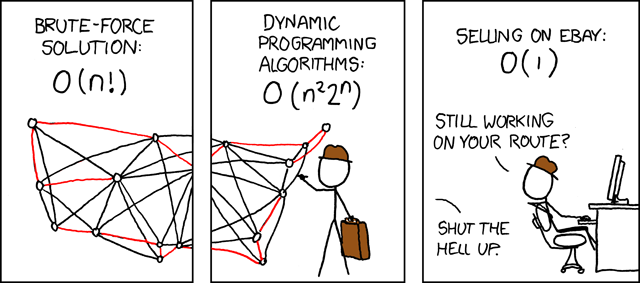
\includegraphics[scale=0.4]{tsp.png}
    \end{center}
\end{frame}

\begin{frame}[plain]{Top-down vs. bottom-up}
    \begin{itemize}
        \item What we have been doing so far is usually called top-down dynamic programming
        \item I.e. you start with the main problem (the top) and split it into smaller problems recursively (down)
        \item In some cases it can be better to do things bottom-up, which is pretty much just the reverse order
        \item Consider for example the fibonacci numbers. Then we'd start at the base cases and count up
    \end{itemize}
\end{frame}


\begin{frame}[plain]{Top-down vs. bottom-up}
    \begin{itemize}
        \item Bottom-up is generally faster, but it has the issue that we have to make sure we iterate through the sub problems in the right order, since recursion doesn't automatically handle that for us
        \item Then why would we use bottom-up?
        \item Sometimes knowing in what order we go through the states can be useful, let's take an example
    \end{itemize}
\end{frame}

\begin{frame}[plain]{Decelerating jump}
    \begin{itemize}
        \item Suppose we have $n$ squares in a row, each containing a value $a_i$. 
        \item We start at the first cell and want to jump through the cells.
        \item If we land on cell $i$ we get $a_i$ points and want to maximize our points.
        \item We can jump to any cell in front of us, but our jump can never go further than our last one.
        \item $n \leq 3000$, $-10^9 \leq a_i \leq 10^9$
    \end{itemize}
\end{frame}

\begin{frame}[plain]{Solution function}
    \begin{itemize}
        \item Let us then find a recursive function describing the answer. 
        \item Let $f(i, j)$ be the maximum score one can get starting at $i$ and using jumps of at most length $j$. Then
            \[f(i, j) = \begin{cases} a_n & \text{ if } i = n \\ \max\limits_{1 \leq k \leq \min(j, n - i)} f(i + k, k) + a_i & \text{ otherwise} \end{cases}\]
        \item Then we have $n^2$ states and it takes linear time to calculate each one. Thus a top-down solution would run in $\mathcal{O}(n^3)$, which is too slow.
    \end{itemize}
\end{frame}

\begin{frame}[plain]{Optimization}
    \begin{itemize}
        \item What about bottom up?
        \item Each $f(i, j)$ only depends on values of $f$ with greater $i$ and lesser $j$, so we can calculate them in increasing order of $j$ and decreasing order of $i$.
    \end{itemize}
\end{frame}

\begin{frame}[plain,fragile]{First implementation}
\scriptsize
\begin{minted}{cpp}
#define INF (1LL << 60)
int main() {
    ll n; cin >> n;
    ll d[n][n], a[n];
    for(int i = 0; i < n; ++i) cin >> a[i];
    for(int i = 0; I < n; ++i) for(int j = 0; j < n; ++j) d[i][j] = -INF;
    d[n - 1][1] = a[n - 1];
    for(int i = n - 2; i >= 0; --i) d[i][1] = d[i + 1][1] + a[i];
    for(int i = 0; i < n; ++i) d[n - 1][i] = a[n - 1];
    for(int j = 2; j < n; ++j) for(int i = n - 2; i >= 0; --i)
        for(int k = 1; k < min(j + 1, n - i); k++) 
            d[i][j] = max(d[i][j], d[i + k][k] + a[i]);
    cout << d[0][n - 1] << '\n';
}
\end{minted}
\end{frame}

\begin{frame}[plain]{Optimized?}
    \begin{itemize}
        \item This is still $\mathcal{O}(n^3)$, so still not good enough.
        \item We note that when we calculate $f(i, j)$ we use the maximum value along the diagonal $f(i + 1, 1), f(i + 2, 2), \dots, f(i + k, k)$.
        \item So we just add a prefix array for the diagonals to calculate those values in $\mathcal{O}(1)$.
        \item This will make the solution $\mathcal{O}(n^2)$, which is good enough, something that couldn't be done with top-down.
    \end{itemize}
\end{frame}

\begin{frame}[plain,fragile]{Fast implementation}
\scriptsize
\begin{minted}{cpp}
#define INF (1LL << 60)
int main() {
    ll n; cin >> n;
    ll d[n][n], e[n], a[n];
    for(int i = 0; i < n; ++i) cin >> a[i];
    for(int i = 0; I < n; ++i) for(int j = 0; j < n; ++j) d[i][j] = -INF;
    d[n - 1][1] = e[n - 1] = a[n - 1];
    for(int i = n - 2; i >= 0; --i) e[i] = d[i][1] = d[i + 1][1] + a[i];
    for(int i = 0; i < n; ++i) d[n - 1][i] = a[n - 1];
    for(int j = 2; j < n; ++j) {
        e[n - j] = max(e[n - j], d[n - 1][j] = a[n - 1]);
        for(int i = n - 2; i >= 0; --i) {
            d[i][j] = e[i + 1] + a[i];
            if(i >= j - 1) e[i - j + 1] = max(e[i - j + 1], d[i][j]);
        }
    }
    cout << d[0][n - 1] << '\n';
}
\end{minted}
\end{frame}


\end{document}
